% !TEX root = DesignDocument.tex


\chapter{Overview and concept of operations}

This section covers an overview of the Crowd Science Mapper. This section will contain information about the purpose, goals, major system components, and technology used.

\section{Team Members and Team Name}
Original team members were Jiasong Yan and Hannah Aker.  Jiasong Yan was removed from the team in January 2016. Project revisions regarding the team member removal can be found in Chapter~\ref{chap:revisions}. Current team members include Hannah Aker. The team is named ``Crowd Science''.

\section{Client}
Clients are Dr. Mengyu Qiao, assistant professor at South Dakota School of Mines and Technology (SDSMT) in the Computer Science Department, and Gail Schmidt, software engineer at Stinger Ghaffarian Technologies (SGT).

\section{Project}
The Crowd Science Mapper project entails creating a proof-of-concept generic crowdsourcing website. This website will demonstrate that crowdsourcing can be accomplished with generic, easy to use interfaces. This interface will allow ordinary users to report information with an event reporting interface and view information with an event viewing interface.

\subsection{Purpose of the System}
As a proof-of-concept project, the purpose of this project is to prove that a generic interface for ordinary users to report events and view events can be created and implemented.

\section{Academic Need}
Currently, there exsist various crowd science mappers designed and implemented for a specific set of events, such as bird sightings and butterfly sightings. Most researchers would need to contract a software designer to implement a crowdsourcing tool for a specific research area, costing time and money. A generic, open-source toolkit or website would provide researchers an easy to use, generic crowdsourcing tool.

\section{Deliverables}
The deliverables in this project will be a proof-of-concept generic crowd sourcing website. This website will feature interfaces for users to view events and report events. The scope of this project does not include moblie applications. 

\section{System Description}

\subsection{Generic Event Reporting}
Ordinary citizens will be able to log in and report events that can then be viewed by researchers, academics and other ordinary citizens. Reports will contain information about the location and time of event, as well as details specific to the type of event.

\subsection{Generic Event Viewing}
Researchers will be able to view event reports in a map representation, with greater event report detail provided below the map. The map will feature pins that show information about the event when hovered over. The detailed list will contain all information about the event reports currently on the map, with an option to show all information in the set of event reports.

\section{Systems Goals}
The goal of this system is to provide a generic crowdsourcing website, that is versatile for any type of data researchers want to research, easy and intuitive enough for any user to report events and view data, and reliable and secure enough for academic use.

\section{System Overview and Diagram}
The webpage will consist of the major components, generic event reporting and generic event viewing. The main page will contain a map and detailed list of events for the selected event set. There will be a button on the main page that will take the user to a reporting interface.  See Figure~\ref{overviewdesign}.

\begin{figure}[tbh]
\begin{center}
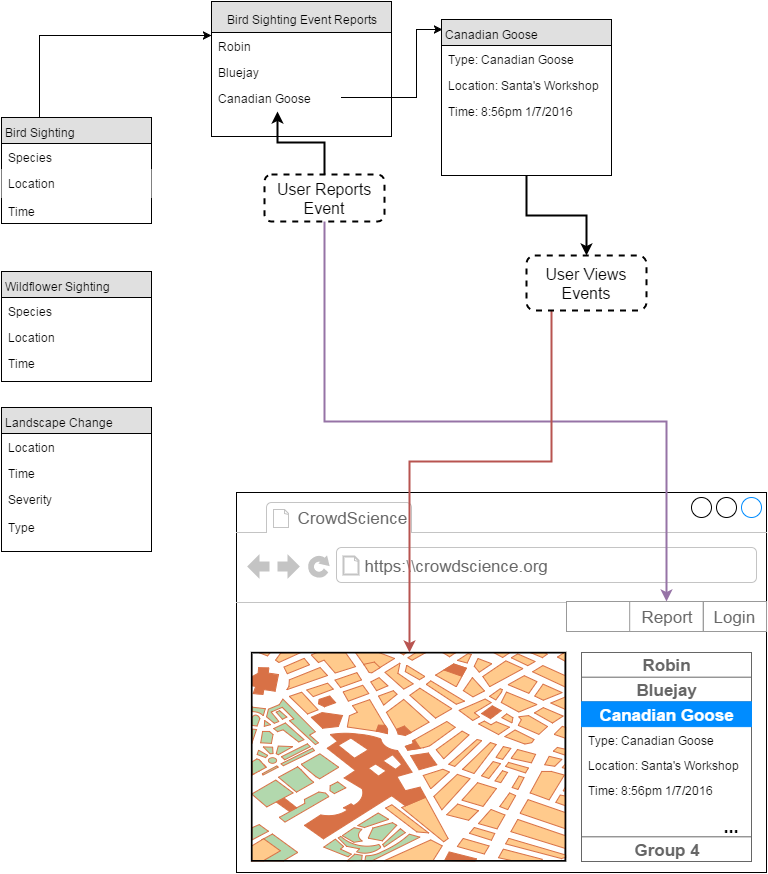
\includegraphics[width=0.75\textwidth]{./figures/overviewdesign.png}
\end{center}
\caption{Design of Crowd Science Main Page\label{overviewdesign}}
\end{figure}

\section{Technologies Overview}
This section contains a list of specific technologies used to develop the system.  See Table~\ref{technologies}.  

\begin{table}[tbh]
\caption{Technologies Used \label{technologies}}
\begin{center}
\begin{tabular}{|>{\raggedright}p{2cm}|>{\raggedright}p{4cm}|>{\raggedright}p{4cm}|>{\raggedright}p{4cm}|}

  \hline
\textit{\textbf{Technology}} &  \textit{\textbf{Description}} & \textit{\textbf{Reference Material}} & \textit{\textbf{System Usage}}\tabularnewline
\hline
 \textit{\textbf{Apache 2.0}} & \textit{Used for website server hosting.} & \textit{\url{http://httpd.apache.org/docs/2.0/}} & \textit{Used to host Crowd Science Mapper website.}\tabularnewline
\hline
 \textit{\textbf{HTML}} & \textit{Hypertext Markup Language, basic webpage scripting language.} & \textit{\url{http://html.net/}} & \textit{Used to tie together JavaScript, PHP, and CSS webpages.}\tabularnewline
 \hline
  \textit{\textbf{JavaScript}} & \textit{More advanced language to create more complex objects.} & \textit{\url{http://html.net/}} & \textit{Used to create more complex objects, such as the event map.}\tabularnewline
 \hline
  \textit{\textbf{PHP}} & \textit{Hypertext Preprocesser, used with HTML to provide stateful webpages.} & \textit{\url{http://html.net/}} & \textit{Used to send and recieve information from the Mongo Database.}\tabularnewline
 \hline
  \textit{\textbf{CSS}} & \textit{Cascading Style Sheet, used to create a unified look and feel for websites.} & \textit{\url{http://html.net/}} & \textit{Used to create look and feel of Crowd Science Mapper.}\tabularnewline
 \hline
  \textit{\textbf{Mongo Database}} & \textit{Used to store information.} & \textit{\url{http://www.mongodb.org/}} & \textit{Used to store user login information and event reports.}\tabularnewline
\hline
\end{tabular}
\end{center}
\end{table}

